\begin{savequote}[\quotewidth]
C\textsubscript{n}H\textsubscript{2n+2} + O\textsubscript{2} $\rightarrow$ CO\textsubscript{2}+ H\textsubscript{2}O + \SI{45}{\kilo\joule\per\gram}\\
CO\textsubscript{2} + H\textsubscript{2}O + h$\nu$ $\rightarrow$ C\textsubscript{6}H\textsubscript{22}O\textsubscript{2} 
\qauthor{Hydrocarbons give heat and sunshine makes sugar}
\end{savequote}

\chapter{Introduction: Climate, fuel and biodiesel} % Main chapter title

\label{Chapter1} % Change X to a consecutive number; for referencing this chapter elsewhere, use \ref{ChapterX}

% ----------------------------------------------------------------------------------------
% SECTION 1
% ----------------------------------------------------------------------------------------

\section{Energy, fuel and the atmosphere}

Industrialized societies depend on reliable sources of energy. For the purpose
of this discussion, the main types of energy are considered to be electricity and
fuels, although they are interconvertible. Fuels for industrialized societies
are predominantly found as underground mineral deposits, from where they are
extracted by mining or drilling. They are found as solids, liquids and gases,
which the energy industry refers to as \keyword{coal}, \keyword{crude oil}, and
\keyword{natural gas}. Because these fuels are of biological origin, deposited
during previous geological eras, and then metamorphosed and preserved by
geological processes, these fuels are commonly referred to as `fossil fuels'.

The large-scale exploitation of fossil fuels started in the middle of the 18th
century, when the plentiful coal from the coalfields of Great Britain drove a
development that is is known to history as the Industrial Revolution. This
development is closely associated with steam engines \autocite{Rosen2012}. The
use of crude oil started in the middle of the 19th century, and is associated
with the development of the automobile \autocite[p. 42]{Watts2005}. The use of
natural gas started in the middle of the 20th century and is associated with the
introduction of gas-fired central heating for homes in cold climates
\autocite{Hanmer2017}. Fossil fuels also serve as feedstock to the chemical
industry, but that topic lies outside the scope of this discussion.

There is no doubt that the use of fossil fuels as an energy source greatly
improved human circumstances. The mechanization of agriculture and the easy
distribution of food by motorized transport have eliminated famine as a natural
disaster \autocite{DeAngelis2007}. The distribution of medical supplies by
motorized transport and the rapid deployment of medical personnel have limited
the impact and spread of epidemics \autocite{Ministere2018}. Heating and cooling
of buildings have increased the habitable zone on earth. Artificial light has
increased the hours available for mental activity, in particular extending the
reach of entertainment, art and education.

However, in the context of chemistry, the uncontrolled use of fuels has at least
two major problems: The first is that it is finite. There is only a finite
amount of fossil fuel on earth. If all of it is extracted it will no longer be a
reliable source of energy, and the existence of industrialized societies and the
complex civilizations that depend on them will be in jeopardy. It is tempting to
think that civilizations would have the foresight to prepare for such an
eventuality, but the historical record shows that societies can collapse when at
the height of their powers \autocite{Diamond2006}.

The second problem with fuels is that they produce \keyword{pollution} wherever
they are produced, processed, transported and used. Pollution is injurious to
the health and well-being of individuals, societies and nature. When pollution
becomes pervasive, it not only degrades society and the environment, but also
negates the benefits brought by the application of energy: modern hospitals are
possible through the intensive application of energy, but if they are filled
with victims of pollution there is no nett benefit.

The first approach to pollution from fuels has been to ignore it. Pictures
from the early industrial revolution shows English towns coated with soot and
choked with smoke \autocite{Flick1980}, and rivers became toxic
sewers \autocite{Halliday2001}.

The development of public health, social responsibility \autocite{Szreter2003}
and an embryonic environmental movement \autocite{Williams1965} lead to
political pressure for the implementation of pollution controls, which
governments gradually introduced and increased in strictness. The first
generation of pollution control offered essentially two options:
concentrate or dilute.

%\footnote{Abatement is also an option, but if economic
%competition is strong then abatement is a natural outcome of the drive towards
%efficiency: every atom of carbon in the fuel not turned into carbon dioxide
%represents lost revenue, hence organic pollutants tend to be minized by economic
%forces. Those of us who saw the fall of the Berlin wall remember the revelation
%of the extreme pollution emitted by Communist industry. The same might not be
%true for other pollutants.}

These two options can be illustrated using the example of a typical South
African coal-fired power station. In such a power station coal is burned to
produce heat, which converts liquid water into high-pressure steam. The steam is
allowed to expand through a turbine, which converts the energy in the steam into
rotary motion that turns an alternator that produces an electric current by
rotating a set of electrical conductors in a magnetic field. The furnaces of
such a power station produce a flow of waste. This waste is an
\keyword{aerosol}: finely divided solids suspended in a mixture of gases.

The solid part is typically separated from the gas-phase part by filter bags and
electrostatic precipitators: the collected material is known as \keyword{fly
ash}. The gas-phase part might be sent through scrubbers to remove some of the
gas-phase pollutants, capturing it in a solid form. The solid part of the power
station's furnace waste has now been concentrated. It is transported to a
storage site, where it is stored indefinitely. It goes without saying that
concentrated pollutants should be encapsulated during storage in some way,
otherwise they just become additional sources of pollution.

The gas-phase part of the pollutant is handled by diluting it. The outlet for
the gas-phase stream of waste is through a tall stack, which ends high above
ground level\footnote{The chimneys of those sooty Victorian towns were not there
to disperse the smoke, but to create a `draft', a flow of air created by the
buoyancy of hot air. The better the draft, the more efficient the fire.}. At
this altitude the wind is strong and steady, which rapidly carries away and
disperses the gases and remaining aerosols.

The dilution of pollutants might seem like an abdication of responsibility, but
it is a reasonable response to pollution. Most pollutants that enter the
biosphere at low enough concentration are broken down into harmless compounds by
sunlight and microbes. This makes dilution a reasonable first attempt at
controlling pollution.

The devil is, of course, in the detail. For example, mercury that finds its way
into the environment is eventually converted by microbes to neurotoxic methyl
mercury, which concentrates in aquatic animals. All rivers in the continental
USA are now polluted by airborne mercury that originate from coal-fired power
stations \autocite{Wentz2014}. Some persistent organic pollutants, which also
concentrate in the food chain, originate from fuel combustion. So while dilution
was a reasonable first attempt at controlling pollution, it is certainly not the
final solution.

The majority of fuels provide their energy as heat, which can be converted into
useful work. This heat is obtained by combining the chemical compounds found in
the fuel with atmospheric oxygen to form compounds with lower internal energy.
The maximum amount of work that can be extracted from a given fuel can be
estimated by examining the Gibbs free energy equation:

\[
	\Delta G = \Delta H - T \Delta S
\]

For a given fuel compound, \(\Delta H\) is determined by the difference
in enthalpy of formation of the product waste compounds and the enthalpy of
formation of the reactant fuel compounds. Since the reactant fuel compounds are
given, \(\Delta H\) is maximized by having product compounds with very low
enthalpies of formations.

To maximize \(\Delta S\), the products should be as disordered as possible. This
implies that \emph{gas-phase} products composed of \emph{small molecules} will
yield more work.

The temperature \(T\) should also be as high as possible.

Because the industrial machinery in economically competitive, capital-intensive
industries is highly efficient, the maximum amount of energy is extracted from
their fuels at the lowest cost. Following Gibbs, the major compounds left over
after extracting the energy from a fuel should have very low enthalpies of
formation and be in the gas phase at the temperature of the process. 

Because all fuels contain carbon as a major component, the extraction of energy
yields compounds containing carbon. Most fuels also contain hydrogen. Reacting
these fuels with the oxygen in air to extract maximal work will therefore
yield water (H\textsubscript{2}O) and carbon dioxide (CO\textsubscript{2}). 

(Of course the argument is not that Victorian engineers designed steam engines
using the Gibbs energy equation, but the variation-selection process
\autocite[Chapter 8]{Vincenti1990} by which engineering improvements accrue would
inevitably drive the development of heat engines fuelled by fossil fuels to emit
large quantities of carbon dioxide gas.)

Water is of course not a pollutant at all, and carbon dioxide is only toxic at
very high concentrations, and therefore, for most of the industrial era, carbon
dioxide was easily dealt with by by diluting it in the atmosphere, where it is
also naturally present at low levels. To the extent that carbon dioxide was
considered a pollutant it was assumed that it would be absorbed by the
biosphere.

Photosynthesis does indeed remove carbon dioxide from the atmosphere, and an
elementary model of the carbon cycle that assumes stability would seem to
indicate that excess carbon dioxide in the atmosphere would be captured by
photosynthesis and sequestered, leaving the carbon dioxide concentration in the
atmosphere stable. Of course this model contains testable assumptions, which
scientists could, and did, test.

The most famous of these tests is probably the ``Keeling Curve''
\autocite{Harris2010}. This is a continuous record of measurements of
concentration of atmospheric carbon dioxide in the pristine air of the Pacific
Ocean. This record starts in 1958 and shows that the carbon dioxide
concentration of the atmosphere is increasing.

Paleoclimatologists have studied the hypothesis that the carbon dioxide
concentration is stable over time. Not only have they found that the carbon
dioxide concentration is \emph{not} stable, they have also determined that the
pre-industrial concentration of atmospheric carbon dioxide was lower than it was
in 1958 \autocite{Petit1999}.

So it is clear that the carbon dioxide concentration in the atmosphere is rising
because the biosphere is not absorbing all the carbon dioxide produced by the
combustion of fossil fuels. The projected concentration of carbon dioxide in the
atmosphere is, however, still not at or even near toxic levels, which might make
the continued dilution of carbon dioxide in the atmosphere seem a viable
disposal method.

Emitted gases, however, do not only have chemical properties and biological
impacts, they also have physical properties. Of concern for the current
discussion is carbon dioxide's absorbance of electromagnetic radiation, in
particular the radiation arriving from the sun, and the radiation from the
earth's surface out to space, both of which must pass through the atmosphere. An
atmospheric molecule can absorb parts of this radiation by having its electrons
excited, or by changing its vibration state. Carbon dioxide is very stable, and
therefore it is electronically excited only by extreme-ultraviolet radiation,
just like the major gases in the atmosphere, molecular nitrogen and molecular
oxygen. It poorly absorbs near-ultraviolet and visible light, which makes it
also similar to the major gases. Because there are dipole moments between the
carbon atom and the oxygen atoms of the carbon dioxide molecule, it is
vibrationally excited by radiation in the infrared region of the electromagnetic
spectrum. Oxygen and nitrogen molecules do not have dipole moments, and
therefore these gases do not absorb infrared radiation strongly. This means that
carbon dioxide will absorb infrared radiation in the atmosphere much more
strongly than the major gases. The energy from the absorbed infrared radiation
is of course turned into vibration, a form of kinetic energy, and this kinetic
energy is randomly distributed among the gases of the atmosphere, appearing as
an increase in temperature as the energy distribution moves towards equilibrium.

The most cursory understanding of the absorption of infrared radiation in the
atmosphere by carbon dioxide therefore seems to say that an increase in the
concentration of carbon dioxide in the atmosphere would lead to a higher average
temperature in the atmosphere. This increase in temperature was first estimated
by Svante Arrhenius in 1896 \autocite{Arrhenius1897}.

(The other major product of extracting energy from fuel is water. Its molecule
also has a dipole moment, and it also absorbs infrared radiation strongly.
However, its intermolecular properties set an upper limit to its concentration:
at high enough concentrations it will either condense into water or crystallize
into ice and precipitate from the atmosphere to end up as surface water.)
Further research has only confirmed that the use of industrial processes that
extract energy from fuel is increasing the amount of carbon dioxide in the
atmosphere by gigatons every year \autocite{Xu2010}, and that this increase is
leading to higher temperatures in the atmosphere. It has also become
increasingly certain that this increase in temperature is inevitable and
significant: it will change the earth's climate\footnote{The atmosphere is in
contact with the hydrosphere, and the two exchange carbon dioxide. The carbon
dioxide diluted in the atmosphere is therefore also diluted in the oceans. This
leads to \keyword{ocean acidification}, a gigaton problem in its own right, but
one that falls outside the scope of this discussion.}. This projected increase
in temperature and the accompanying change in global climate is bound to have
impact on societies within the lifetime of people alive today, and a larger
impact on future generations. Some of these projected changes are incompatible
with the maintenance of the complex civilizations that are supported by
industrialized societies \autocite{IPCC2014}.

Scientists do not inhabit ivory towers, and their research is funded by public
money in the expectation that the resulting science will benefit their
societies. As the understanding of carbon pollution grew, it became obvious to
scientists that industrialized societies could not just continue diluting
gigatons of carbon dioxide in the atmosphere, and they alerted policymakers. The
iconic moment of this development was the testimony of Dr James E. Hansen, at
the time director of NASA's Goddard Institute of Space Studies, before the
Senate of the US Congress in 1988 \autocite{Shabecoff1988}. In the same year the
scientists of the world came together and established the Intergovernmental
Panel on Climate Change (IPCC) to create a coherent body of knowledge to inform
decision-making. The IPCC has so far produced a series of five Assessment
Reports, which assess the science of climate change, its impacts, and ways to
mitigate it \autocite{Allen2014}.

(Carbon dioxide is not the only greenhouse gas and the IPCC reports consider
each in detail, but because the other gases are not produced in significant
quantities by fuels and the energy industry they fall outside the scope of this
discussion.)

Industrialized societies require reliable supplies of energy to function.
Currently that requirement is met through the use of fossil fuels. But the
future health and well-being of humanity depends on ending the use of fossil
fuels. Therefore, it is in the best interest of industrialized societies to
create plans to reduce the dependence on energy from fossil fuels and exploit
alternative energy sources. Industrialized societies, however, are also in
economical competition with each other. This means that any society that spends
resources on risky, expensive alternative sources of energy risks falling into a
competitive disadvantage, and there is a surfeit of short-sighted politicians
who will take advantage of this risk to create fear and so prevent planning for
and investment in changes in energy production and use\footnote{The impact of
political corruption is not negligible but will not be discussed further.}.

Fortunately there are enough leaders who have vision, and based on the
recommendations of the IPCC the governments of the world have come together to
create the UNFCCC. The United Nations Framework Convention On Climate Change is
an international agreement that structures the response of nations to limit
their emissions of greenhouse gases. Two international treaties have been agreed
to so far: the Kyoto Protocol in 1997 \autocite{Kyoto1997} and the Paris
Agreement in 2015 \autocite{Paris2015}.

These agreements attempt to reduce the amount of carbon dioxide released into
the atmosphere by dividing the cost of reducing emissions fairly. While the
Kyoto Protocol invoked a complex carbon credit trading scheme, in the Paris
Agreement nations pledge to reduce emissions of carbon dioxide into the
atmosphere, and each is free to do so in a way that suits them best.

The Republic of South Africa is a signatory to the Paris Agreement, and
therefore the country is legally bound to limit and reduce its emissions of
carbon dioxide and other greenhouse gases. The country has so far promised to
stop increasing emissions between 2020 and 2025 \autocite{INDC2016}.

% ----------------------------------------------------------------------------------------
% SECTION 2 --------------------------------

\section{Carbon footprints and carbon neutrality}

Ending the emission of carbon dioxide by industrialized societies is an exercise
in balancing effort with consequences. Every reduction in carbon dioxide
emissions must necessarily have an effect on the economy, and conversely, every
change in economic activity will have an effect on carbon dioxide emissions.

A rational, discerning society in searching for ways to reduce carbon dioxide
emissions will therefore attempt to change their economy in such a way that the
emission of carbon dioxide is limited or reduced. But in most societies there
are many ways to reduce carbon dioxide emissions, and decisions have to be made
on which ones to implement. Such decisions must be based on sound information,
and one way to generate that information is a discipline called \keyword{life
cycle analysis} (LCA). Life cycle analysis can yield rigorously-calculated data
and comparisons, but it is a very general method. For analyses that are very
similar and differ only in context, it is possible to develop simplified,
standardized life-cycle analysis tools.

One such tool is the \keyword{carbon footprint}. Every economic activity in an
industrialized society emits greenhouse gases. These emissions might  be far
removed from the activity in space and time. A familiar example of this is the
use of electricity: At the moment I'm using an electronic computer to compose
this paragraph and electric light illuminates the desk I'm working at here in my
office in Pretoria. One can name the activity ``academic writing." The
electricity that powers the computer and the lamps are generated hundreds of
kilometres from here, most of it on the Mpumalanga Highveld, in coal-fired power
stations that emit carbon dioxide in the process. So my activity is far removed
from the associated emissions \textbf{in space}. But even before the coal was
burned, the machines that mined it and transported it to the power station
emitted carbon dioxide, so my activity is also removed from the emissions
\textbf{in time}. The sum of all these emissions connected with my activity
constitutes the carbon footprint of my activity.

Although carbon footprinting is conceptually straightforward, it is analytically
rigorous and computationally complex. But there are standard protocols
\autocite{WRI2004} that can be followed, so that carbon footprints from
different activities and different organizations are transparent and comparable.
Once an organization's activities have been footprinted, the organization can
examine its operations and look at ways to change activities that will reduce
that footprint. If my university, for example, decides to install solar panels
on the roof of my building, and use the electricity to illuminate my office, the
activity of academic writing will now most likely have a reduced carbon
footprint, because solar electricity usually has a lower carbon footprint than
coal-derived electricity.

To prevent a climate disaster, at some point industrialized societies will have
to change all their activities until they no longer emit any greenhouse gases.
Such activities will have carbon footprints of zero, and will be known as
`carbon neutral activities'. There are also activities that are nett removers of
carbon from the atmosphere, which would be `carbon negative'.

In reality, in industrialized societies there are very few carbon neutral
activities. Even if I'm just sitting quietly in a pristine nature reserve, the
food I am digesting and metabolizing has a positive carbon footprint: carbon
was emitted to fix nitrogen from the air, which was used as fertilizer to help
grow the food I ate, and is now in the proteins of my body. The very calcium and
phosphorus in my bones were sourced from mines that were powered by fossil
fuels. 

\section{Internal combustion engines.}

An organization that calculates carbon footprints for its activities quickly
learns that a major source of emissions is transport. Most transport in
industrialized societies is powered by \keyword{internal\hyp{}combustion
engines}. (They are called `internal\hyp{}combustion' engines because the
chemical transformation that extracts the energy from the fuel is internal to
the engine. This is in contrast to the power station steam turbines mentioned
earlier, where the extraction of the chemical energy from the fuel happens
outside of the engine. The engine is the device that produces the mechanical
energy.) These engines are usually powered by liquid fuels derived from crude
oil, although some designs run on gas, and of course in South Africa Sasol and
PetroSA supply liquid fuels derived from coal and natural gas.

This discussion will use the term \keyword{noxious pollution} to describe
pollution that is directly harmful to humans and \keyword{carbon pollution} to
describe pollution that leads to climate disruption.

The simplest way to reduce an activity's carbon footprint is to use the fuel
that drives that activity more efficiently. Fortunately market forces are
aligned with this, because more efficient use of a fuel also reduces running
costs. Discussing engine designs therefore almost always invokes
\keyword{efficiency}. Efficiency of an engine is calculated by dividing the
\keyword{output power} \(P_{out}\) by the \keyword{input power} \(P_{in}\). The
greek letter \(\eta\) is used as a symbol for efficiency:

\[ \eta = \frac{P_{out}}{P_{in}} \]

Conservation of energy dictates that the output power cannot be more than the
input power, and therefore \(\eta \leq 1\). The power is `lost' to two factors:
firstly entropy, as dictated by the Second Law of Thermodynamics, and secondly
losses, such as friction.

\subsection{Scaling and efficiency} \label{par:scaling}

The larger an engine is, the more efficient it is, and the improvement is
logarithmic. Three factors improve efficiency in larger engines
\autocite{Brown2017}:

\begin{enumerate}

\item Longer residence time: In larger engines, the reacting fuel spends more
time in the engine. This gives reactions more time to reach equilibrium, and
hence more energy can be extracted.

\item Smaller surface area to volume ratio: The volume of an engine increases
with the cube of its linear dimension, but the surface area increases with the
square of its linear dimensions. This means that larger engines have a smaller
surface-to-volume ratio than smaller engines. Since losses take place at the
surface, the loss per unit volume is therefore larger for smaller engines than
it would be for larger engines of the same type. If the losses in larger engines
are comparatively smaller, we can expect larger engines to be more
efficient than smaller ones. 
  
\item Larger Reynolds number: The Reynolds number is a number that predicts the
onset of turbulent flow, and is calculated from the viscosity, velocity and a
characteristic linear dimension.  The higher the Reynolds number, the higher the
likelihood of turbulent flow. Turbulent flow promotes mixing, which leads to
improved combustion and hence higher efficiency. The larger the engine, the
larger the characteristic linear dimension, and therefore the higher the
likelihood of turbulent flow.

\end{enumerate}

From the viewpoint of reducing carbon pollution, one should therefore aim to use
a few large engines rather than a multitude of small engines.

\subsection{Engine design and thermodynamic cycles.} \label{par:efficiency}

The final design of a successful internal combustion engine is determined by the
variation-selection process described by Vincenti \autocite{Vincenti1990}. Such
a design sufficiently satisfies a wide range of requirements. These requirements
might be explicitly expressed in documentation or they may be implied or they
may be practical. These requirements would include, but are not limited to,
capital cost, running cost, maintenance cost, noise, sound\footnote{In 1994 the
motorcycle manufacturer Harley-Davidson attempted to trademark the distinctive
sound of the engines they install in their motorcycles \autocite{ODell2000}.},
ease of maintenance, power output, emissions, surface finish, weight, mounting
method, size, supply chain capability, shape, colour, fuel availability,
operating temperature, altitude tolerance and torque.

From designers' attempts to fulfil these requirements arise the myriad of
different engine designs, delivering anything from milliwatts to megawatts of
power to anything from model aircraft to oil tankers. Fortunately for
researchers who study engine efficiency, there are only a few conceptual systems
that explain how the internal combustion engines convert the chemical energy of
the fuel into mechanical work.

The principles on which the different engines operate are named `cycles',
because the way they convert heat into work can be describe in terms of a series
of events that are repeated endlessly. The concept of a cycle is further
entrenched because it is customary to explain the thermodynamic processes
involved using a \textbf{PV diagram}, a research tool that shows the changes of
state of the working fluid during engine operation.

Theoretical thermodynamic cycles are useful because they can predict the
performance of heat engines, allowing for comparison. In particular, it allows
for comparison with theoretical maxima. The maximum efficiency of a heat engine
is delivered by an engine running on the Carnot cycle. This describes a
hypothetical engine that uses only reversible processes to extract useful work
from the temperature difference between two reservoirs of heat. It has been
shown that the Carnot cycle offers the maximum possible heat extraction, and
that the maximum efficiency (\(\eta_{C}\)) is determined solely by the temperature
difference between the hot (\(T_h\)) and the cold (\(T_c\)) reservoirs.

\[
	\eta_{C} = 1 - \frac{T_c}{T_h}
\]

The Carnot cycle, however, can only deliver an infinitesimal amount of work,
because the heat transfer must be reversible, and therefore infinitesimal. A
more realistic maximum efficiency is given by the Chambadal-Novikov efficiency
(\(\eta_{CN}\)) \autocite{Hoffmann2008}:

\[
	\eta_{CN} = 1 - \sqrt{\frac{T_c}{T_h}}
\]

This theoretical efficiency takes into account the irreversible processes that
are inevitable in engines delivering finite amounts of power.

Barring revolutionary new discoveries and inventions, there will be only three
thermodynamic cycles and their corresponding internal combustion engines on the
market as we enter the low-carbon era.

\subsubsection{Otto engine and Otto cycle}

The oldest of the internal combustion engines is the Otto engine. It is named
after Nikolaus Otto, who developed the first working engine of this kind in 1876
\autocite[Chapter 9]{Cummins1989}. In South Africa these engines are usually
called `petrol engines`. In the Otto engine, a homogeneous mixture of
atmospheric air and vaporized fuel is compressed. This mixture is then ignited
by an electric spark. The energy released by the chemical reaction between the
oxygen in the air and the fuel vapour causes the temperature of the compressed
air to rise, and consequently also the pressure. If this --- now hot --- gas is
allowed to expand in an expandable vessel, the motion of the vessel can be
captured to perform useful work. Once the useful work is extracted, the vessel
can be collapsed again to expel the exhausted air, and re-filled with a
compressed air/fuel vapour mixture. This completes the cycle (See Figure
\ref{fig:otto-cycle}). The expandable vessel is usually in the form of a
cylinder and piston, with the piston connected to a crank that drives a shaft
that transfers the work from the engine to the machine being powered.

\begin{figure}
\centering
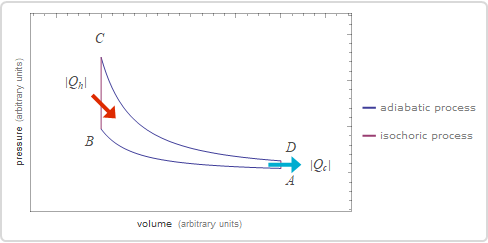
\includegraphics[width=\textwidth]{Figures/otto-cycle}
\decoRule

\caption[The Otto cycle]{The pV diagram of the thermodynamic Otto cycle. The
isochoric heat addition step (BC) corresponds to the burning of the homogeneous
air-fuel mixture. Work is extracted from the engine during the adiabatic
expansion CD \autocite{Wolfram|Alpha2019Otto}. }

\label{fig:otto-cycle}
\end{figure}

(These legs of the cycle are only loosely related to the `strokes' of a
four-stroke engine, and should not be confused for them.) 

The theoretical efficiency of the Otto cycle is given by 

\begin{equation}
	\eta = 1 - (\frac{1}{r^{\gamma-1}})
\label{eqn:otto-efficiency}
\end{equation}

where \(r\) is the \keyword{compression ratio}, \( \frac{V_1}{V_2} \), and
\(\gamma\) is the heat capacity ratio, which can be considered a constant for
the purposes of this discussion \autocite{Wolfram|Alpha2019Otto}.

This means that the efficiency of an Otto engine can be improved by increasing
the degree of compression of the intake air before combustion. 

\subsubsection{Diesel cycle}

In the diesel engine, named after Rudolf Diesel who demonstrated the first
engine of this type in 1897 \autocite[Chapter 14]{Cummins1989}, air is
compressed, and then a finely divided solid or liquid fuel is injected into the
system. The fuel then reacts with the oxygen in the air. The energy released in
the reaction appears as a higher temperature in the gas, and --- following
Gay-Lussac's Law --- the pressure of the gas rises. If the gases expand in the
confines of a collapsible vessel, useful work can be extracted from expansion of
the vessel. Once the work has been extracted, the vessel can be collapsed again
to remove the now inert ('exhausted') gas and prepare for receiving the next
charge of air, completing the cycle. The theoretical cycle used to analyse the
performance of the diesel engine is called the Diesel cycle. (See Figure
\ref{fig:diesel-cycle})

\begin{figure}
	\centering
	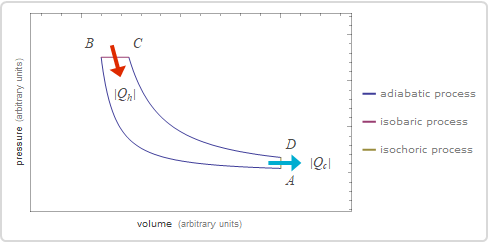
\includegraphics[width=\textwidth]{Figures/diesel-cycle}
	\decoRule

	\caption[The Diesel cycle]{The pV diagram of the thermodynamic Diesel cycle. The
	isobaric process BC corresponds to the combustion of the finely divided fuel
	particles in air. Work is extracted from the engine both during this process and
	during the adiabatic process CD. \autocite{Wolfram|Alpha2019Diesel}}

	\label{fig:diesel-cycle}
\end{figure}

The Diesel cycle differs from the Otto cycle in the heat addition step. In the
Otto engine, the heat addition takes place when the homogeneous air/fuel mixture
combusts. This combustion takes place in a short space of time during which the
engine parts move only a negligible distance. Hence the pressure rises rapidly.
In the diesel engine, the fuel is injected into a volume of compressed air,
where it combusts. (There is no separate ignition source: the temperature of the
adiabatically compressed air is higher than the fuel's \keyword{auto-ignition
temperature}, so that the fuel ignites upon injection. While this is another
difference between the two engines, it is of second-order importance when
discussing thermodynamic cycles.) Because the combustion takes place at the
surface of fuel particles, the combustion rate is lower than the combustion rate
of the homogeneous mixture in the Otto cycle. Hence the rising temperature is
balanced by the motion of the engine, and the heat addition is essentially
isobaric.

The theoretical efficiency of the Diesel cycle is given by Equation
\ref{eqn:diesel-efficiency}

\begin{equation}
	\eta = 1 - \frac{1}{r^{(\gamma - 1 )}}(\frac{\alpha^{\gamma}-1}{\gamma(\alpha-1)})
\label{eqn:diesel-efficiency}
\end{equation}
 
where \(\alpha\) is the \keyword{cut-off ratio} and \(\gamma\) is the compression ratio.

The term \( \frac{\alpha^{\gamma}-1}{\gamma(\alpha-1)} \) is always larger
than \(1 \), and therefore, when we compare equation \ref{eqn:diesel-efficiency}
with equation \ref{eqn:otto-efficiency} it is clear that for a given
compression ratio the Diesel cycle is always less thermally efficient than the
Otto cycle. 

However, at high compression ratios Otto engines start suffering from
\keyword{knocking}. This is the phenomenon of the homogenous air/fuel mixture
detonating instead of burning smoothly. The shock waves from this detonation
will damage the engine and lead to faster wear. (The \keyword{octane number} of
a fuel indicates the compression ratio it can accommodate.) Because Diesel
engines do not suffer from this problem, they can, and usually are, designed to
operate at higher compression ratios than Otto engines.  Otto engines normally
operate with a compression ration of up to 9:1, whereas diesel engines have
compression ratios of up to 25:1. This makes Diesel engines significantly more
efficient than Otto engines.

\subsubsection{Gas turbines and the Brayton cycle}

The third internal\hyp{}combustion engine important to industrialized society is
the \keyword{gas turbine}. Gas turbines are used rarely in road transport, more
often in marine and stationary applications, but thousands take to the sky every
day, propelling aircraft carrying billions of airline passengers every year
\autocite{Morris2017}.

The first gas turbines were developed during wartime urgency to deliver pure jet
thrust for military aircraft, but this proved to be an inefficient use of the
available energy. Most modern turbine engines drive a shaft to extract
rotational work. This shaft might drive a bypass fan (as used in airliner engines), a
propeller (as used in smaller, low-speed aircraft), or a shaft which might drive
a helicopter rotor or an electrical generator.

In operation, a gas turbine compresses air with one or more compressor stages.
The compressed air passes through a combustion chamber, where fuel is added and
combusted. As the now hot gases expand they pass through one or more turbine
stages, which is connected to drive the compressor and the output shaft, which
extracts work from the system. After the gas has passed through the turbine it
returns to atmospheric pressure, optionally doing work on the engine in the form
of thrust.

The theoretical thermodynamic cycle that is customarily used to analyse the gas
turbine is called the Brayton cycle, named after George Brayton, who
successfully manufactured a reciprocating engine based on this cycle. (See
Figure \ref{fig:brayton-cycle}) Such engines are no longer manufactured
\autocite[Chapter 10]{Cummins1989}.

\begin{figure}
	\centering
	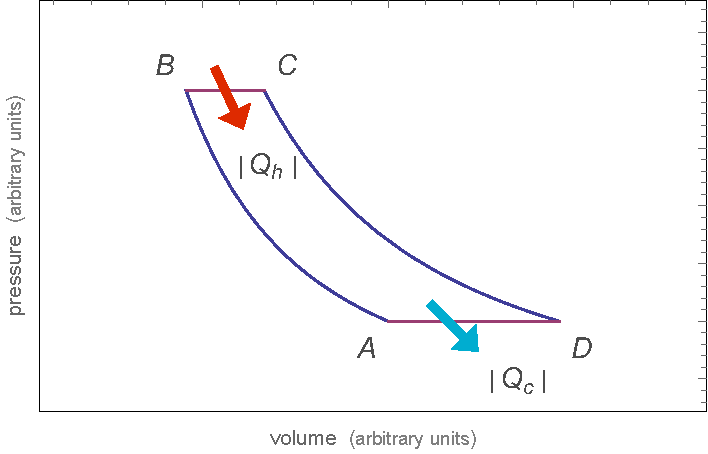
\includegraphics[width=\textwidth]{Figures/brayton-cycle}
	\decoRule
	
	\caption[The Brayton cycle]{The pV diagram of the thermodynamic Brayton cycle.
	In the gas turbine the continuous combustion of the injected fuel and free
	expansion of the air through a turbine means that the heat addition (BC) is
	isobaric. Work is extracted during the adiabatic expansion process CD
	\autocite{Wolfram|Alpha2019Brayton}.}
	
	\label{fig:brayton-cycle}
\end{figure}

The efficiency of the Brayton cycle is given by equation
\ref{eqn:brayton-efficiency} 

\begin{equation}
	\eta = 1 - \frac{T_{1}}{T_{2}} = 1 - (\frac{ P_{1} }{ P_{2} })^{(\frac{\gamma-1}{\gamma})}
\label{eqn:brayton-efficiency}
\end{equation}

where \(\gamma\) is the compression ratio \autocite{Wolfram|Alpha2019Brayton}.

Because the fuel is continuously added to the compressed air and the combustion
takes place in a heterogeneous mixture, gas turbines do not suffer from
`knocking' and therefore there is no upper limit to the compression ratio. The
main figure determining the efficiency of the engine is the turbine inlet
temperature, (\textit{i.e.} the outlet temperature of the combustion chamber)
which reaches \SI{1600}{\celsius} in modern engines.

\subsection{Noxious pollution from internal combustion engines. }

Carbon pollution is not the only pollution emitted by internal combustion
engines. There is also noxious pollution, which affects the societies in which
they are used. There are ways to reduce or eliminate such pollution, but the
implementation of such measures affect the efficiency of the engine. Noxious
pollution from internal\hyp{}combustion engines come from different sourc\-es
and have different effects:

\subsubsection{Incomplete combustion}
\label{sec:IncompleteCombustion}

The combustion reactions in internal\hyp{}combustion engines are very fast, but
they are never at equilibrium. This means that at the end of a cycle, the
exhaust gases expelled from the engine contains, besides the carbon dioxide,
also chemical intermediates and unreacted fuel molecules. Unreacted fuel is a
noxious pollutant in its own right, but when it is released into the environment
chemical reactions induced by sunlight produce \keyword{ozone}, a reactive
oxygen species that cause respiratory problems in victims of pollution
\autocite{Davidson1998}.

Some of the fuel-like pollutants from internal\hyp{}combustion engines are not
present in the fuel. These compounds are formed in a process that might be
called \keyword{pyro-synthesis}. They are themselves more stable than the
compounds from which they originate, but not as stable as the combustion end
products, carbon dioxide and water. Because they are themselves quite stable,
they require high temperatures to combust, which might not be achieved before
they leave the engine as waste. Notable pollutants from this source are the
policyclic aromatic hydrocarbons (PAH) and, if trace amounts of chlorinated
substances are present in the fuel, dioxins.

One of the products of pyro-synthesis is particles of soot. These particles are
agglomerations of nano-sized particles of pure, amorphous carbon. The
agglomerations might include adsorbed PAHs and acids. Soot particles are very
stable and only react at very high temperatures. Diesel engines in particular
have a reputation for producing soot \autocite{Mohankumar2017}.

The final pollutant that can be classed as originating from partially combusted
fuel is carbon monoxide. It forms readily when fuels are burned in oxygen-poor
environments. Modern, well-maintained engines rarely cause acute carbon monoxide
poisoning \autocite{Reumuth2018}, but chronic exposure to low levels of
environmental carbon monoxide has harmful effects \autocite{Wright2002}.

\subsubsection{Contaminants and additives.}

Crude oil and coal contains not only carbon and hydrogen, but also other
elements, most notably sulfur and nitrogen. Depending on the refining process,
these elements might find their way into fuels. Organic nitrogen and sulfur will
easily oxidize and form stable oxides, yielding energy. Once outside the engine,
however, the volatile oxides will dissolve in any atmospheric water and form
acids \autocite{Duncan2016} that contribute to acid rain.

Fuel manufacturers add additives to fuels for various reasons, such as boosting
octane rating or preventing corrosion. The prime example of additives as a
source of noxious pollution was tetraethyllead, which was added to petrol as an
octane booster. The emitted lead compounds were shown to be neurotoxic
pollutants, and its use was phased out \autocite{Needleman2000}.

\subsubsection{Side-reactions}

Most internal combustion engines use atmospheric air as oxidant. This air
consists of \SI{21}{\percent} oxygen, and \SI{78}{\percent} nitrogen. Nitrogen
is very stable and inert at atmospheric temperatures and pressures, but at high
temperatures and pressures it can react with oxygen. These reactions produce the
oxides of nitrogen: NO, NO\textsubscript{2}, NO\textsubscript{3},
N\textsubscript{2}O, and N\textsubscript{2}O\textsubscript{5}, collectively
called \nox. These oxides can participate in the cycle that causes a from of
pollution called \keyword{photochemical smog}. They will also dissolve in
atmospheric water and form acids: this might happen far from the point of
emission, resulting in \keyword{acid rain}.

\subsection{Mitigating pollution from internal\hyp{}combustion engines.}
 
Pollution from internal combustion engines is a social ill, and most governments
have regulations in place to limit and reduce this pollution. Engine and fuel
manufacturers are working hard to reduce this pollution.

The noxious pollution from internal combustion engines can be reduced by various
improvements, but there are three complementary approaches: fuel formulation
\autocite{Gertler1999}, exhaust gas cleanup \autocite{Braun2018} and engine
management \autocite{Reif2015}.

\subsubsection{Fuel formulation}
\label{sec:FuelFormulation}

Adding oxygenates improves the octane rating of fuel and reduces \nox formation
in Otto engines, and governments regulate the amount of sulfur in diesel fuel to
reduce the amount of emitted sulfur oxides.

\subsubsection{Exhaust gas cleanup} \label{par:cleanup}

Exhaust gases from internal combustion engines can be ``cleaned'', and there are
two approaches. The first is catalytic conversion, in which the exhaust gases
that contain the pollutants are passed over a catalyst bed. The catalyst (a
proprietary formulation of platinum, palladium and/or rhodium), adsorbs the
uncombusted volatile organic carbons, and oxidizes them. It simultaneously
catalytically decomposes \nox to molecular nitrogen and oxygen. Secondly, filter
systems can be used to remove particulate matter.

\subsubsection{Engine management} \label{par:engine-management}

As described above, the main source of noxious pollution from
internal\hyp{}combustion engines is uncompleted or undesired chemical reactions,
and is not fundamental to the operation of the engine. By carefully managing the
engine system, noxious pollution can be reduced. 

The only mature engine management technology is the oxygen or `lambda' sensor,
which measures the oxygen in the exhaust gases. Such a sensor, coupled to an
engine-management computer, allows the me\-ter\-ing of the exact amount of fuel
need\-ed for op\-ti\-mum combustion \autocite{Frauhammer2014}.

A newer technology is known as \keyword{exhaust gas recirculation} (EGR). This
mixes the intake air of the engine with exhaust gases, effectively diluting the
oxygen. This reduces peak temperatures, and thereby \nox formation.

In \keyword{stratified charge} engines the distribution of fuel in the volume of
intake air is controlled by selective fuel injection. Carefully injecting the
fuel at the right place at the right time can allow for higher compression
ratios without inducing pinging. \keyword{Lean-burn} engines are Otto engines
that use extremely high air to fuel ratios.

Electronic engine management systems result in much more efficient and
less-polluting engines than non-managed `mechanical' engines, but because
engines for automotive applications endure such a wide range of operating
conditions, they can at best achieve a compromise between power, efficiency and
emissions. It was this unsatisfactory compromise that lead to the Volkswagen
emissions scandal: manufacturers chose to cheat on emissions tests rather than
admit to the relatively poor performance of a managed engine optimized for low
emissions \autocite{Mansouri2016}.

\subsubsection{Efficiency implications}

Attempts to mitigate noxious pollution from internal\hyp{}combustion engines
mostly lead to losses in efficiency. For example:

\begin{itemize}

\item Exhaust gas flow through catalytic converters and filters dissipates
energy that could have been used to perform work.
  
\item The engines cannot approach their theoretical maximum efficiencies,
because reducing \nox emissions is handled by limiting maximum combustion
temperatures.

\item \nox reduction catalysts require the presence of hydrocarbons,
\textit{i.e.} incomplete reactions, which implies that not all energy is
extracted from the fuel.

\item Every treatment system added to the engine adds weight to the vehicle, which
reduces payload and hence the total efficiency.

\end{itemize}

Before carbon dioxide pollution was a concern, it made sense to accept lower
efficiencies as a necessary cost of reducing noxious pollution, but in a
low-carbon future we cannot just continue trading less noxious pollution for
more carbon dioxide production.

\subsection{Avoiding pollution from internal\hyp{}combustion engines} \label{par:carbon-neutral}

The efficiency and cleanness of internal\hyp{}combustion engines have
dramatically increased over the last century, and more improvements are being
implemented. But these improvements have not been fundamental to the engines in
any way, and have been driven mostly by government regulation, at the cost of
increased complexity and a higher purchase price.

It would seem obvious that it would be a good idea to introduce alternative
technologies. 

\subsubsection{Electrification}

In principle, there is nothing special about internal\hyp{}combustion engines:
they are not an end in themselves. They mere\-ly deliver a source of torque,
which can be coupled to machinery to do useful work. Before the industrial era
such torque was available from windmills and waterwheels, and today an
alternative is the electric motor.

Electric motors are engines that use the interaction between electric current
and magnetic fields to deliver useful torque to drive machines. Because they use
electricity as a source of energy, they have no noxious emissions where they
operate. Because they are not heat engines, their efficiencies are not subject
to the Carnot limit, and efficiencies exceeding 95\% are standard \autocite{Li2012}.

Electricity, of course, is not necessarily carbon-neutral. Most electricity is
generated in power plants that use fossil fuels as a primary source of energy.
But because these plants are huge, and efficiency scales logarithmically with
size, the energy output by the electric motor has a similar or lower carbon
footprint than an equivalent internal\hyp{}combustion engine
\autocite{Doucette2011}. Electricity grids are also increasingly being fed by
solar and wind power, which are carbon-neutral at source. These renewable plants
are also smaller and more flexible than their behemoth fossil-fuel counterparts,
with lower capital costs and extremely low running costs. Hence, in a low-carbon
future, there is every reason to support or mandate the use of electrical motors
for stationary applications wherever possible.

In automotive applications, \textit{i.e.} in cases where the engine is used to
move itself in addition to some form of \keyword{payload}, the application of
electric motors is more demanding. In this case it is not easy to bring the
electricity to the motor, although electric trains and buses fed by overhead
conductors are splendid examples of electrified transport. So for electric
vehicles to use the existing road network, they need to carry a source of
electricity with them.

This source of electricity can be a either a chemical \keyword{storage battery},
or a \keyword{fuel cell}. In a chemical battery power from the grid is stored in
the form of reversible electrochemical reaction, and in a fuel cell the chemical
energy from a fuel is directly converted into electricity. There are fuel cells
that can use hydrogen as a fuel, and fuel cells that can use methanol as a fuel.
(It goes without saying that the hydrogen and the methanol need to be sourced
from low-carbon sources for fuel cells to count as low-carbon energy sources.)

The storage and transport of hydrogen remain hurdles to the large-scale adoption
of hydrogen-fuelled automobiles, although a market seems to be developing for
hydrogen-fuelled electric trains \autocite{theguardian_2018}. Hydrogen fuel cells
emit no carbon or noxious pollution at point of use.

Direct methanol fuel cells can react methanol with atmospheric oxygen in an
electrochemical cell to yield electricity, with carbon dioxide
as a waste product. Little is known about possible noxious pollution.

At this time it seems that the electrification of road transport will be by
chemical batteries. Lithium-ion batteries can now store enough energy and
deliver enough power to make electric motor vehicles practical and attractive
\autocite{Hayes2011}, and some governments are considering plans to no longer
allow the production of passenger vehicles propelled by internal-combustion
engines \autocite{Burke-Kennedy2018, Reuters2018, Gabbatiss2018}.

\subsubsection{Carbon-neutral fuels} 

Another way to avoid the carbon pollution associated with internal-combustion
engines is to change the fuel. Not all fuels are fossil fuels, and it is
possible to use fuels that are carbon neutral, and in some cases carbon
negative.

Apart from using hydrogen in a fuel cell, as described above, \keyword{hydrogen}
can also be used as a fuel in Otto engines, because it will combust in air to
yield heat. The emissions are water and \nox. Presently there are no
hydrogen-fuelled Otto engines on the market.

Methanol is a common product of the fossil fuel industry, but work is underway
to produce methanol by reducing carbon dioxide using solar energy. Such
\keyword{solar methanol} might be used in direct conversion fuel cells, or in
internal\hyp{}combustion engines.

It is possible to harness the energy contained in the reduced carbon in
biological materials and use it as fuel. These fuels are known as
\keyword{biofuels}.

\section{Biofuels}

Biological processes are an integral part of the carbon cycle, because
photosynthesis in plants reduces carbon dioxide in the atmosphere to sugars,
which are converted by plant physiology into structural cellulose and other
metabolites. The prototypical biofuel is wood, used in all societies for cooking
and heating. This familiarity makes biofuels seem an obvious and viable source
of energy, but details matter, and switching from fossil fuels to biofuels to
reduce carbon footprints of human activities is not a simple choice.

Firstly, the efficiency of photosynthesis is notoriously low: not above a few
per cent \autocite{Simkin2019}, whereas the efficiency of a modern,
mass-produced silicon-based solar \keyword{photovoltaic} (PV) panel can exceed
\SI{20}{\percent} \autocite{Green2019}. In general, if mechanical power is
required it will be much more efficient to capture solar energy in a PV panel
and use it to power an electric motor than to produce a biofuel and use it to
fuel an internal-combustion engine.
 
Secondly, increased biofuel production has numerous impacts on the environment
and society which cannot be ignored. Discussing all the factors that need to be
studied to make such a decision is outside the scope of this work, but as an
example a report prepared for stakeholders in the Netherlands
\autocite{Smeets2006} uses the following criteria:

{\itshape
\begin{itemize}
  \item GHG [greenhouse gas] emissions – the use of biofuels should cause reductions of GHG emissions. The
comparison should be done regarding the average use of fossil fuels, considering the life
cycle of fossil and biofuels (\textit{i.e.}, well-to-wheel basis) and in case of biofuels reduction
should be at least 30\%
 \item Impacts over food supply – the production of biomass for energy must not endanger the
food supply and other local biomass applications. The analysis should be developed
considering possible changes of land use in the region of biomass production.
 \item Biodiversity – Biomass production must not affect protected or vulnerable biodiversity.
 \item The basic criteria are that violation of national laws and regulations are unacceptable.
 \item Local environmental effects – Principles include (a) soil and soil quality, that must be
retained or even improved, (b) ground and surface water supply, that must not be polluted.
 \item Local economic effects – The production of biomass must contribute towards local
prosperity.
 \item  Social well-being – The production of biomass must not decrease the well-being of local societies. 
\end{itemize}
}

Nevertheless, there are cases where using biofuels is an option that reduces the
impact of energy use on the environment.

\subsection{Bio-gas}

Anaerobic bacteria can convert carbon compounds of biological origin to methane.
This methane is identical to the methane obtained from natural gas, and can be
used for the same applications, including fuelling Otto engines and gas
turbines. This technology has been applied since the industrial revolution, when
some streetlamps in England were fuelled with bio-gas \autocite[p.
448]{Klass1998}.

An excellent application for the use of bio-gas is waste remediation. Waste
material from the agri-food industry can be highly polluting if not handled
responsibly, emitting noxious chemicals into water and the potent greenhouse gas
methane into the atmosphere. When used as feedstock for bio-gas production it
reduces carbon pollution by capturing methane and displacing natural gas and
also prevents water pollution \autocite{Venter2014}.

\subsection{Bio-ethanol}
\label{sec:BioEthanol}

The technology to convert sugars or starch from plant materials into ethanol by
microbial fermentation is as old as civilization. The products of this process
are beer and wine.  Beer and wine can best be described chemically as aqueous
solutions of sugars, ethanol, flavourants and colourants, with or without
suspended solids, and are of no use as fuels. It was not until the 8th century
CE that Persian and Arab scientists mastered the art of distillation and
purified ethanol \autocite{Modanlou2008}, and it was not until Pasteur that
yeast was seen as a living organism and it was understood that ethanol is a
product of its metabolism \autocite{Barnett2000}. It is unclear when ethanol was
first used as a fuel, but its flammability must have been noticed by the first
distillers. By 1838 pure ethanol was common enough to be used in alcohol lamps as a
source of heat in the chemical laboratory \autocite{Griffin1838}, and by the
1850s it was a major component of lamp oil used for illumination in the USA
\autocite{Abebe2008}. Ethanol as a fuel for internal combustion engines has a
clear start date: in 1826 Samuel Morley was granted a patent for an engine
designed to use ethanol as fuel \autocite[p.79]{Cummins1989}.

The industrial production of ethanol as a fuel is a technologically advanced
process and an active research field. A paper \autocite{Cardona2007}
reviewing the process technology of producing bio-ethanol written in 2007 had
garnered 644 citations by January 2019. The industrial production of ethanol
consists of three steps:

\begin{enumerate}
  \item Fermentation
  \item Distillation
  \item Dehydration
\end{enumerate} 

The fermentation step is the biological process by which the yeast organism
\textit{Saccharomyces cerevisiae} converts the sugar and starch in the
biological material to ethanol and carbon dioxide. This needs to be done in a
sterile environment to prevent contamination by other micro-organisms.

The distillation step is the physical process of separating the produced alcohol
from the aqueous mixture in which it is produced. This generally produces an
\keyword{azeotropic mixture} that contains \SI{95.6}{\percent} ethanol
\autocite{Kumar2010}.

While the processes of fermentation and distillation of ethanol for fuel are in
principle the same as that of producing alcoholic beverages, the emphasis of the
processes are very different. In the beverage industry the emphasis is on the
development of complex flavours and a consistent, recognizable drinking 
experience. In the fuel industry the emphasis is on efficiency and throughput.

To produce fuel-grade ethanol from the distilled azeotrope, dehydration is a
necessary third step. This step can be implemented by various distillation
processes that add a third compound, but in most modern plants the water is
removed by adsorption onto molecular sieves \autocite{Kumar2010}.

\subsubsection{Brazilian ethanol}

Brazilian sugar-cane ethanol is an integral part of the country's energy
network. In that country most Otto-engine vehicles have `flex-fuel' engines,
which can be fuelled with any blend of ethanol and petrol. The industry is
regarded as sustainable \autocite{Smeets2006}.

\subsubsection{US maize}

US maize ethanol is primarily blended with petrol to meet legislative
requirements of oxygenates in fuels. The production of maize is water-intensive
and the fermentation process is carbon-intensive. The US ethanol from maize has
a poorer energy balance and larger carbon footprint than Brazilian ethanol from
sugar cane, but has a smaller water footprint \autocite{Mekonnen2018}.

Ethanol can fuel Otto engines and gas turbines. 

\subsection{Fischer-Tropsch fuel from biomass}
\label{sec:FT}

It is possible to heat woody biomass with steam in a low-oxygen environment to
produce synthesis gas, which can be the converted to a mix of fuel products in
the well-known Fischer-Tropsch catalytic process. Such a  fuel could be called a
bio-fuel, but it's production would be difficult to reconcile with the
principles of \keyword{green chemistry}, described in Section
\ref{sec:GreenChemistry}.

\subsection{Hydrotreated vegetable oil: ``Green diesel''}
\label{sec:GreenDiesel}

The petroleum industry has developed a collection of chemical processes, such as
hydrogenation, oxygenation and cracking. This collection of processes can be
applied to vegetable oils to produce a fuel for diesel engines and gas turbines.
This path is being followed by the aviation industry \autocite{Chiaramonti2014}.

\subsection{Biodiesel}

Oils and fats have been used as fuels since antiquity, most obviously as a fuel
for lamps: olive oil has been identified as the fuel used in lamps dating from
around 600 CE \autocite{Kimpe2001}, and at the Paris World Fair in 1900 Rudolf
Diesel demonstrated an engine that ran on peanut oil \autocite{Knothe2010}.

During the energy crisis of the 1970s which caused high prices and shortages of
crude oil, the South African government looked at alternative sources of fuel.
Experiments were done with sunflower oil as a fuel for agricultural tractors,
but the formation of carbon deposits injector nozzles was an intractable
problem. Seeing that the clogging of the injectors might be caused by the high
viscosity of the sunflower oil as a fuel, the \keyword{transesterification} of
the oil was implemented, replacing the glycerol in the sunflower oil with
methanol (See Figure \ref{fig:Transesterification}). This created an oily liquid
with a lower viscosity, which proved to be a trouble-free alternative to diesel
fuel \autocite{VanNiekerk1980}. With the easing of the energy crisis the
interest in this technology waned.

\begin{figure}[hptb]
	\centering
	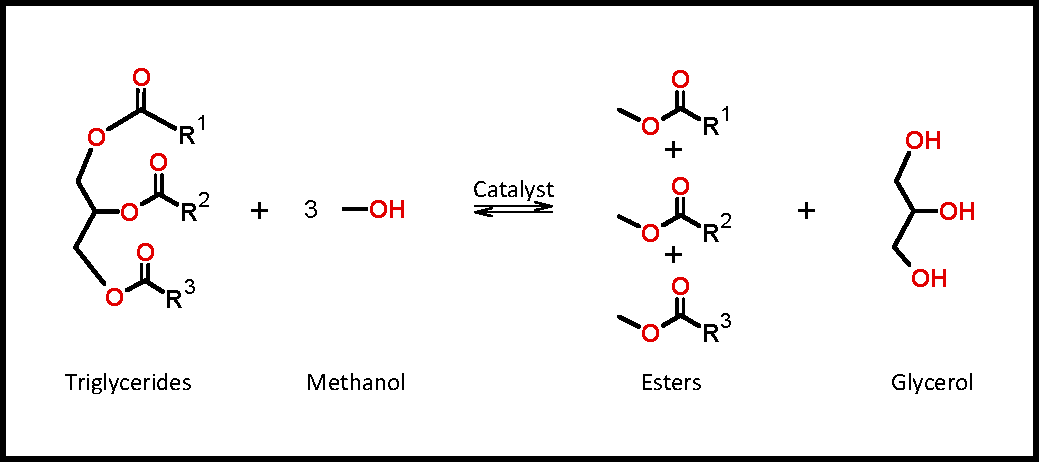
\includegraphics[width=\textwidth]{Figures/Transesterification.pdf}
	\decoRule
	
	\caption[Transesterification]{Transesterification: the chemical reaction that
	converts vegetable oils into biodiesel}
	
	\label{fig:Transesterification}
\end{figure}

Such a transformed oil is termed \keyword{biodiesel}. It consists primarily of a
mixture of fatty acid methyl esters, often abbreviated into the acronym FAMEs.
Compared to ethanol, biodiesel production is relatively simple, the main method
sharing much with the ancient technology of making soap. This simplicity makes
the production of biodiesel attractive to small and decentralized manufacturing,
and consequently governments consider biodiesel production an attractive
proposition: it can create job opportunities in rural populations and it can
create a stable market for farmers who produce vegetable oil crops.

Biodiesel is not yet carbon neutral: the methanol used to create the methyl
esters is a product of the petroleum industry, and therefore biodiesel emissions
contribute to global warming. But replacing fossil diesel fuel with biodiesel
results in a nett reduction of carbon emissions, with the future possibility of
replacing fossil-derived methanol with carbon-neutral bio-methanol
\autocite{Shamsul2014}.

% ----------------------------------------------------------------------------------------
% SECTION 4 --------------------------------
\section[The significance of biodiesel ]{Conclusion: the significance of
biodiesel and its quality control.}

In a complex technical, economic and social environment it is likely that there
will always be a need that can be best met by internal combustion engines. The
decision on the type of engine and the decision on the fuel for that engine are
not independent, as Cummins reminds us \autocite{Cummins1989}:

\begin{quotation}
``Our generation faces a similar challenge in a real liquid fuel energy shortage
that will come within the lifetime now living. As we plunge into the seeking of
solutions to our dilemma, we must never forget that \textit{an engine and the
fuel it consumes are inseparable partners}; the one cannot progress without the
full cooperation of the other. This precept is vital to the planning of future
powerplants, since an engine's design determines its fuel and binds us to our
future resource requirements.''
\end{quotation}

The variation-selection process by which real engineering progress is `blind':
the combination of factors that make a design successful is not known at the
start of a development \autocite{Vincenti1990}. But scientific knowledge
provides guidance to engineering design in the form of insight into processes
and theoretically achievable targets for performance. Using the scientific
knowledge we have today, we can risk a forecast: if society is determined that
its carbon footprint should be reduced with minimal noxious pollution, then the
application of internal combustion engines would tend towards the following:

\begin{enumerate}
  
  \item Larger: Because larger engines are more efficient than smaller engines,
  larger engines would be preferred. (See section \ref{par:scaling})
  
  \item Low-carbon: The preferred engine would be fuelled by carbon-neutral
  fuels. (Section \ref{par:carbon-neutral})
  
  \item Constant speed: Engines are most efficient when they can work at
  constant load. (Section \ref{par:engine-management})
  
  \item Efficient: Engines with high efficiency should be preferred, which
  implies engines with high compression or pressure ratios. (Section
  \ref{par:efficiency})
  
  \item Cleanup: The exhaust should be amenable to cleanup, \textit{i.e.} the
  exhaust gases of the fuel-engine system should not contain compounds that are
  incompatible with available converter or filter technologies. (Section
  \ref{par:cleanup})
     
\end{enumerate} 

From this it should be clear that the optimal engine of the future will not be
an Otto engine, because it will always have a limited compression ratio and its
catalytic exhaust cleanup will always require stoichiometric air:fuel ratios,
which puts bounds to efficiency increases.

Because it is the most efficient engine, the gas turbine will play an important
role. However, its exhaust temperature is very high, which begs for energy
recovery to increase the efficiency of the system. Such systems are already seen
in the \keyword{combined cycle gas turbine} (CCGT). But energy recovery systems
are not light and small, so their best application outside aerospace (where the
excess heat is utilized as thrust) appears to be stationary electricity
generation.

To reduce the carbon footprint of automotive applications, the best engine may
be a large diesel engine with exhaust cleanup to remove \nox and soot, fuelled
with a carbon-neutral fuel.

In choosing between hydrotreated vegetable oil and biodiesel as a fuel, it is
most likely that biodiesel will have a lower carbon footprint. Refinery
operations are energy intensive, which might add to the carbon footprint of the
fuel. Refineries are not usually near the point of use, so that transport will
also add to its carbon footprint. The carbon emissions of locally-produced
biodiesel are comparatively low, which means that its carbon footprint will tend
to be smaller. (At this point it is important to note that these observations
are not definitive: carbon footprints are not predicted, they must be
calculated.)

Buying large, highly efficient diesel engines with sophisticated management
systems and exhaust cleanup require high capital investment. In an economically
competitive environment they therefore need to bring reliable returns, which
implies high availability, as measured by frequency of breakdown and length of
time between maintenance stops. Such high reliability can only be achieved if
the engine builder understands the fuel-engine system well and it behaves
predictably.

In a low-carbon future, therefore, well-characterized biodiesel might be
expected to play a central role in non-electric ground transport and other
industrial applications where electrification is not possible.

\section{Conclusion: the role of chromatography.}

The development of the fuel-engine systems depends heavily on the chemical
characterization of fuels and engine emissions, and chromatography has always
played a central role: some of the earliest researchers developing gas
chromatography were employees of a petrochemical company
\autocite{Keulemans1955}.

This thesis explores the possibility of applying comprehensive two-dimensional
(supercritical fluid × gas) chromatography (SFC×GC) to the chemical analysis of
biodiesel for characterization and quality control.

The next chapter (Chapter \ref{Chapter2}) focuses on the use of supercritical
carbon dioxide as extractant and chromatographic mobile phase. Chapter \ref{Chapter3}
explores the technical standards applicable to biodiesel offered for sale in
South Africa, and then focuses on the prescribed chromatographic methods.
Chapter \ref{Chapter4} and Chapter \ref{Chapter5} focus on the chromatographic
instrumentation developed for SFC×GC, and Chapters \ref{Chapter6} and
\ref{Chapter7} show the results obtained when biodiesel and biodiesel blends are
analysed using the developed SFC×GC instrumentation. Chapter \ref{Chapter8}
shows a chromatogram that illustrates the promise of SFC×GC-FID when the carbon
dioxide mobile phase is modified by the addition of organic solvents.